\documentclass[11pt,a4paper,twocolumn]{article}

% === Core Packages ===
\usepackage[margin=2cm]{geometry}
\usepackage[utf8]{inputenc}
\usepackage[T1]{fontenc}
\usepackage{times}
\usepackage{amsmath,amssymb}
\usepackage{graphicx}
\usepackage{booktabs}
\usepackage{float}
\usepackage{enumitem}
\usepackage{tikz}
\usepackage{pgfplots}
\pgfplotsset{compat=1.18}
\usetikzlibrary{arrows.meta,shapes.geometric,positioning,calc,decorations.markings,fit,backgrounds}

% === Citation (IEEE style) ===
\usepackage[numbers,sort&compress]{natbib}
\bibliographystyle{IEEEtranN}

% === Hyperref ===
\usepackage[hidelinks]{hyperref}
\usepackage{xurl}

% === Settings ===
\setlength{\parindent}{1em}
\setlength{\parskip}{0.3em}

% === Title ===
\title{\textbf{Decentralized Reputation Network:\\A Framework for Natural Societal Organization}}
\author{Pavel Kudrna\\Prague, Czechia\\Draft v1 --- March 2026}
\date{}

\begin{document}
\maketitle

% ============================================================
% ABSTRACT
% ============================================================
\begin{abstract}
Das Gerechtigkeitsempfinden---die Überzeugung, dass Unrecht wiedergutgemacht und Verdienst belohnt wird---ist die stärkste zusammenhaltende Kraft der Gesellschaft. Wenn zentralisierte Regierungsinstitutionen dieses Empfinden nicht liefern können, weil die Kosten der Durchsetzung eines Rechts den Wert des Rechts selbst übersteigen, erodiert der gesellschaftliche Zusammenhalt. Die gegenwärtigen institutionellen Strukturen versagen bei der Beilegung einer bedeutenden Klasse von Streitigkeiten systematisch auf dieselbe Weise, wie die Zentralplanung bei der Ressourcenallokation versagt: durch Informationsasymmetrie, fehlende Rückkopplungsschleifen und die Loslösung der Entscheidungsträger von den Folgen ihrer Entscheidungen. Diese Arbeit stellt ein Reputationsnetzwerk (Reputation Social Network, RSN) vor: eine dezentrale, unbestechliche, zensurresistente Kommunikationsschicht, die auf dezentralen Identifikatoren (Decentralized Identifiers, DIDs) aufbaut und pseudonymen Teilnehmern ermöglicht, Reputationsinformationen über reales Verhalten zu veröffentlichen, zu verifizieren und zu konsumieren. Der Kernmechanismus beruht auf drei Gestaltungsprinzipien: (1)~einer asymmetrischen Kostenstruktur, bei der das Lesen von Reputationsdaten kostengünstig ist, das Schreiben jedoch nachweisbaren Aufwand erfordert; (2)~einem nichtdeterministischen Protokoll zur Auswahl von Verifizierern auf Basis von konsistentem Hashing, das radikale Behauptungen durch eskalierende Iterationskosten bepreist; und (3)~einem marktgetriebenen Modell der Reputationsautorität, bei dem private Verifizierer ihre angesammelte Reputation auf die Richtigkeit der von ihnen bestätigten Behauptungen setzen. Die daraus resultierende Architektur erzeugt eine emergente Meritokratie ohne zentrale Koordination und ermöglicht einen schrittweisen, umkehrbaren Migrationspfad von bestehenden staatlich verwalteten Systemen.
\end{abstract}

% ============================================================
% 1. INTRODUCTION
% ============================================================
\section{Einleitung}

\subsection{Das Problem des zentralisierten Vertrauens}

Moderne Regierungsführung beruht auf einer grundlegenden Annahme: dass zentralisierte Institutionen Vertrauen zwischen Fremden in großem Maßstab vermitteln können. Gerichte entscheiden Streitigkeiten. Register beglaubigen Eigentum. Regulierungsbehörden setzen Standards durch. Diese Institutionen wurden in einer Zeit entworfen, in der Informationen knapp waren, Kommunikation langsam war und die Delegation von Autorität an eine zentrale Stelle der einzig machbare Koordinationsmechanismus war. Zentralisierte Regierungsführung versagt jedoch aus denselben strukturellen Gründen wie die Zentralplanung: Informationsasymmetrie, fehlende Rückkopplungsschleifen und die Loslösung der Entscheidungsträger von den Folgen ihrer Entscheidungen.

Die Annahme versagt beispielsweise dann, wenn die Kosten der institutionellen Vermittlung den Wert der Streitigkeit übersteigen. Man stelle sich einen Mieter vor, der entdeckt, dass seiner Mietwohnung ein gesetzlich vorgeschriebenes Zertifikat über die elektrische Sicherheit fehlt---ein Zustand, der eine unmittelbare Lebensgefahr darstellt. Das gesetzliche Recht des Mieters, vom Vertrag zurückzutreten, ist eindeutig. Dennoch übersteigen die Kosten der Durchsetzung dieses Rechts über das Gerichtssystem den Geldwert der Kaution und der geschuldeten Schäden, selbst unter Einbeziehung einer möglichen gesetzlichen Entschädigung~\cite{czcourtfees}. Die rationale Reaktion besteht darin, den Verlust hinzunehmen und auszuscheiden.

Dies ist kein pathologischer Sonderfall. Es ist die Standarderfahrung bei einer bedeutenden Klasse von Streitigkeiten, bei denen der Schaden real ist, aber der finanzielle Einsatz unter die Schwelle fällt, ab der eine institutionelle Durchsetzung wirtschaftlich rational wird. Das Ergebnis ist ein System, das strukturell schlechte Akteure begünstigt: Wer anderen in Mengen unterhalb dieser Schwelle schadet, kann ungestraft handeln, weil die Kosten der Rechtssuche auf die geschädigte Partei fallen.

Das obige Beispiel stammt aus dem Rechtsumfeld des Autors---dem tschechischen zivilrechtlichen System. In anderen Rechtstraditionen---dem auf Präzedenzfällen beruhenden Common Law, dem Gewohnheitsrecht, gemischten Systemen---versagt die Gerechtigkeit auf unterschiedliche Weise und in unterschiedlichem Ausmaß, je nach den kulturellen und verfahrenstechnischen Besonderheiten der jeweiligen Rechtsordnung. Die Leser werden vermutlich vergleichbare Beispiele aus ihrem eigenen Umfeld erkennen. Strukturell universell ist das Muster: Streitigkeiten, deren Wert unter die Schwelle einer wirtschaftlich rationalen Durchsetzung fällt, enden damit, dass der Verlust von der geschädigten Partei getragen wird. Das RSN verspricht keine perfekte Gerechtigkeit---es verringert lediglich den strukturellen Vorteil, den schlechte Akteure genießen, wenn die institutionelle Durchsetzung unwirtschaftlich ist.

\subsection{Warum bestehende Lösungen zu kurz greifen}

\textbf{Frameworks für dezentrale Identität (DID)}~\cite{did2022} bieten kryptografische Mechanismen für ein selbstbestimmtes Identitätsmanagement, konzentrieren sich jedoch in erster Linie auf die Identitätsverifizierung, ohne die umfassendere Frage der Verhaltensreputation zu behandeln.

\textbf{Soulbound Tokens (SBTs)}~\cite{weyl2022} erfassen die Erkenntnis, dass Reputation nicht übertragbar ist, sind jedoch auf eine Blockchain-Infrastruktur mit Skalierbarkeitsbeschränkungen angewiesen und behandeln nicht die wirtschaftlichen Anreize, die den Informationseintrag steuern. Verwandte Konzepte wie Verdiensttoken (z.\,B. Liberland) teilen eine ähnliche Philosophie, bleiben jedoch an spezifische rechtsordnungsgebundene Rahmenwerke gebunden.

\textbf{Dezentrale autonome Organisationen (DAOs)}~\cite{buterin2014} implementieren Governance über Smart Contracts, replizieren jedoch plutokratische Dynamiken, bei denen der Einfluss proportional zum Kapital ist. Quadratisches Abstimmen~\cite{buterin2019} mildert dies teilweise, begrenzt jedoch die praktische Verbreitung. DAOs stehen zudem vor dem grundlegenden \emph{Orakel-Problem}: Smart Contracts können reale Zustände nicht zuverlässig verifizieren, ohne eine vertrauenswürdige externe Quelle, und dieses Problem hat innerhalb der Blockchain-Architektur keine allgemeine Lösung.

Kein bestehendes System vereint Dezentralisierung, Zensurresistenz, Pseudonymität, nachweisbare Eintrittskosten und emergenten Konsens.

\subsection{Beiträge}

Diese Arbeit leistet die folgenden Beiträge:
\begin{enumerate}[nosep]
\item Definition des \textbf{Reputationsnetzwerks (Reputation Social Network, RSN)}, eines dezentralen Protokolls, das das DID-Framework um die Unterstützung eines bilateralen Reputationsaustauschs erweitert.
\item Ein \textbf{nichtdeterministisches Protokoll zur Auswahl von Verifizierern} auf Basis von konsistentem Hashing~\cite{karger1997}.
\item Das \textbf{Prinzip des teuren Radikalismus}, das Behauptungen entsprechend ihrer Distanz zum Netzwerkkonsens über drei sich verstärkende Kostenkanäle bepreist.
\item Ein \textbf{Modell der reputablen Autorität} mit asymmetrischen Anreizen, bei dem eine falsche Bestätigung katastrophal mehr kostet als legitime Gebühren.
\item Ein \textbf{schrittweiser Migrationspfad} über eine parallele fiskalische Infrastruktur.
\end{enumerate}

% ============================================================
% 2. DESIGN PRINCIPLES
% ============================================================
\section{Gestaltungsprinzipien}

Die RSN-Architektur wird durch fünf nicht verhandelbare Gestaltungsprinzipien eingeschränkt.

\textbf{Kontinuität und Evolution.} Das System koexistiert mit bestehenden Institutionen während einer Übergangszeit von unbestimmter Länge. Der Übergang muss in jeder Phase umkehrbar sein.

\textbf{Freiwilligkeit und Verantwortung.} Die Teilnahme ist freiwillig, aber Freiwilligkeit ist mit Verantwortung verbunden: Ein Teilnehmer, der die Kontrolle über eine institutionelle Funktion übernimmt, übernimmt zugleich die damit einhergehenden Pflichten.

\textbf{Vielfalt und kulturelle Neutralität.} Der Konsens entsteht aus bilateralen Interaktionen, nicht aus voreingestellten Regeln, die von den Systemgestaltern auferlegt werden.

\textbf{Widerstandsfähigkeit und Zensurresistenz.} Die Kosten der Zensur des Netzwerks müssen die Kosten seiner Duldung übersteigen. Nur ein vollständiger Totalitarismus---zu ruinösen politischen und wirtschaftlichen Kosten---kann das System unterdrücken.

\textbf{Konsens und Durchsetzung.} Das System integriert menschliche Neigungen zu Kleinlichkeit, Boshaftigkeit und vergeltender Genugtuung als tragende Merkmale. Fehlverhalten ist nicht verboten; es wird bepreist.

% ============================================================
% 3. SYSTEM OVERVIEW
% ============================================================
\section{Systemübersicht}

\subsection{Reputationsnetzwerk}

Das RSN ist eine dezentrale Peer-to-Peer-Kommunikationsschicht, in der Teilnehmer verifizierbare Informationen über reales Verhalten austauschen. Seine definierenden Eigenschaften sind: dezentrale und unzensierbare Infrastruktur; pseudonyme Teilnahme über DIDs; asymmetrische Kostenstruktur (Lesen ist günstig, Schreiben ist teuer); kryptografische Verifizierbarkeit; und \textbf{Standardunterstützung}---maschinenlesbare Formate für Informationen, die durch das Netzwerk propagiert werden, für Dienste, die von Autoritäten angeboten werden (Zusammenstellung von Behauptungen, Bestätigung, Zeugendienst), und für das Richtlinienformat einschließlich der Regeln zur Bewertung der Reputation der Gegenpartei und zur Einschätzung des Risikos einer Richtliniendiskrepanz (zwischen deklariertem und tatsächlichem Verhalten).

\subsection{Architektonische Komponenten}

Das RSN besteht aus vier primären Komponenten (Abb.~\ref{fig:architecture}):
\begin{enumerate}[nosep]
\item \textbf{DID-Schicht.} Teilnehmeridentitäten mit deklarierten Regeln, Reputationsmetadaten und Netzwerkrouting.
\item \textbf{Behauptungsprotokoll.} Strukturiertes Format zur Veröffentlichung von Aussagen über reale Ereignisse.
\item \textbf{Verifizierungsnetzwerk.} Dezentrales Protokoll zur Zuweisung von Verifizierern mittels konsistentem Hashing.
\item \textbf{Reputationsaggregationsschicht.} Dienste, die menschenlesbare Reputationszusammenfassungen erzeugen.
\end{enumerate}

\begin{figure}[ht]
\centering
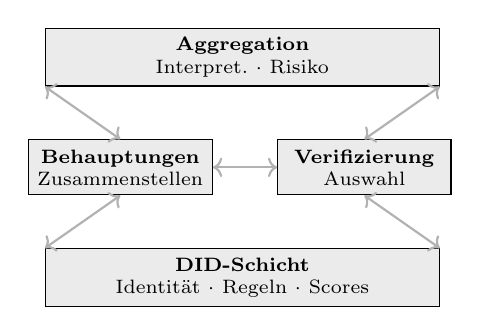
\begin{tikzpicture}[
    layer/.style={draw, minimum height=0.7cm, align=center, font=\scriptsize, fill=black!8},
    arr/.style={<->, thick, gray!60}
]
\node[layer, minimum width=5cm] (agg) at (0,2.8) {\textbf{Aggregation}\\Interpret.\ $\cdot$ Risiko};
\node[layer, minimum width=2.2cm] (claim) at (-1.55,1.4) {\textbf{Behauptungen}\\Zusammenstellen};
\node[layer, minimum width=2.2cm] (verif) at (1.55,1.4) {\textbf{Verifizierung}\\Auswahl};
\node[layer, minimum width=5cm] (did) at (0,0) {\textbf{DID-Schicht}\\Identität $\cdot$ Regeln $\cdot$ Scores};

\draw[arr] (agg.south west) -- (claim.north);
\draw[arr] (agg.south east) -- (verif.north);
\draw[arr] (claim.east) -- (verif.west);
\draw[arr] (claim.south) -- (did.north west);
\draw[arr] (verif.south) -- (did.north east);
\end{tikzpicture}
\caption{Vierschichtige RSN-Architektur.}
\label{fig:architecture}
\end{figure}

\subsection{Teilnehmerrollen}

An einer Verifizierungstransaktion sind bis zu sechs unterschiedliche DID-Rollen beteiligt (Abb.~\ref{fig:roles}): \textbf{Aussteller} ($DID_I$, erstellt und übermittelt die Behauptung), \textbf{Subjekt} ($DID_S$, die DID, um die es in der Behauptung geht---kann mit dem Aussteller zusammenfallen), \textbf{Autorität} ($DID_A$, bestätigt die Behauptung gegen eine Gebühr; kann auch Zeugendienste anbieten---\emph{optional}), \textbf{Zeuge} ($DID_{W_{1..n}}$, inkognito überwachende Instanz der Ehrlichkeit des Verifizierers über Challenge-Codes---\emph{optional}), \textbf{Verifizierer} ($DID_V$, algorithmisch ausgewählt, um die Behauptung zu veröffentlichen) und das \textbf{RSN} (das Netzwerk, in dem verifizierte Behauptungen veröffentlicht werden). Jede Rolle kann an eine andere DID delegiert werden (Abschnitt~7.4). Eine Autorität bündelt üblicherweise Bestätigung mit Zeugendiensten, aber die beiden Funktionen sind logisch unabhängig.

\begin{figure}[ht]
\centering
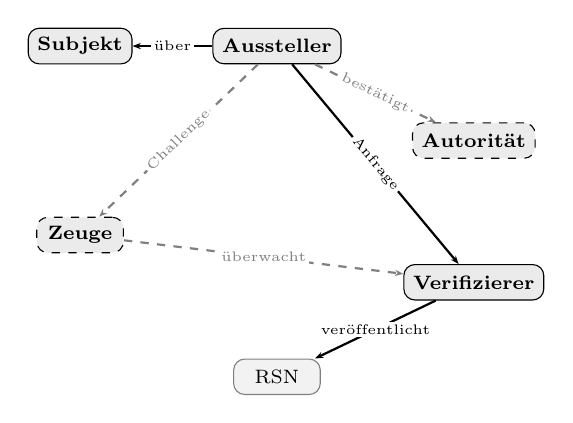
\begin{tikzpicture}[
    role/.style={draw, rounded corners, minimum width=1.1cm, minimum height=0.45cm, align=center, font=\scriptsize, fill=black!8},
    opt/.style={draw, rounded corners, minimum width=1.1cm, minimum height=0.45cm, align=center, font=\scriptsize, fill=black!8, dashed},
    arr/.style={-{Stealth[length=3pt]}, thick},
    oarr/.style={-{Stealth[length=3pt]}, thick, dashed, gray},
    lbl/.style={font=\tiny, fill=white, inner sep=1pt}
]
\node[role] (I) at (0,2.4) {\textbf{Aussteller}};
\node[role] (S) at (-2.5,2.4) {\textbf{Subjekt}};
\node[opt] (A) at (2.5,1.2) {\textbf{Autorität}};
\node[opt] (W) at (-2.5,0) {\textbf{Zeuge}};
\node[role] (V) at (2.5,-0.6) {\textbf{Verifizierer}};
\node[role, fill=black!5, draw=gray] (N) at (0,-1.8) {RSN};

\draw[arr] (I) -- node[lbl] {über} (S);
\draw[oarr] (I) -- node[lbl,sloped] {bestätigt} (A);
\draw[oarr] (I) -- node[lbl,sloped] {Challenge} (W);
\draw[arr] (I) -- node[lbl,sloped] {Anfrage} (V);
\draw[oarr] (W) -- node[lbl] {überwacht} (V);
\draw[arr] (V) -- node[lbl] {veröffentlicht} (N);
\end{tikzpicture}
\caption{DID-Rollen in einer Verifizierungstransaktion. Gestrichelt = optional (Autorität, Zeuge).}
\label{fig:roles}
\end{figure}

\subsection{Unbestechlichkeit: Vier Kräfte}

Die Unbestechlichkeit des RSN entsteht nicht aus einem einzigen Mechanismus, sondern aus vier gleichzeitig wirkenden Kräften. Keine ist für sich allein ausreichend; erst ihre Kombination macht einen Korruptionsversuch wirtschaftlich irrational.

\textbf{Unvorhersehbares Ziel.} Der Verifizierer für jede Behauptung wird nichtdeterministisch durch konsistentes Hashing ausgewählt (Abschnitt~5.3). Ein Angreifer kann keinen bestimmten Verifizierer für eine Bestechung vorab ins Visier nehmen, weil die Identität des Verifizierers eine Funktion des Inhalts der Behauptung und vorheriger Iterationen ist, nicht der Wahl des Ausstellers.

\textbf{Reputationshebel---langsam hoch, schnell runter.} Reputation kann nur schrittweise gewonnen werden, durch anhaltendes konsistentes Verhalten. Sie kann jedoch in einer einzigen betrügerischen Bestätigung katastrophal verloren gehen (Abschnitt~6.2). Diese Asymmetrie bedeutet, dass jahrelang angesammelte Reputation durch eine einzige unehrliche Bestätigung zerstört werden kann; die optimale Strategie bleibt, verdächtige Behauptungen abzulehnen.

\textbf{Öffentliches Versprechen.} Jeder DID-Inhaber deklariert öffentlich seine Richtlinie---einen maschinenlesbaren Satz von Regeln, deren Einhaltung er sich verpflichtet. Eine Abweichung zwischen der Deklaration und dem tatsächlichen Verhalten ist erkennbar und wird als Reputationsvergehen bepreist, das schwerer wiegt als der zugrunde liegende Verstoß (Abschnitt~7.3). Heuchelei ist daher kostspieliger als direkte Unehrlichkeit.

\textbf{Asymmetrie der Angriffskosten im Netz.} Die Kosten der Zensur oder Destabilisierung des Netzwerks wachsen nichtlinear mit der Größe und Dichte des Netzwerks, während die Kosten seiner Duldung konstant bleiben. Damit sich Zensur lohnt, müsste ein zentralisierter Akteur sie über das gesamte Netzwerk anwenden---was Maßnahmen erfordern würde, die in keinem Verhältnis zu einem denkbaren Nutzen stehen (Abschnitt~10).

% ============================================================
% 4. DECENTRALIZED IDENTITY MODEL
% ============================================================
\section{Modell der dezentralen Identität}

\subsection{DID mit besonderen Eigenschaften}

Das RSN erweitert die W3C-DID-Core-Spezifikation~\cite{did2022} um: \textbf{Deklarierte Regeln} (maschinenlesbare Verhaltensverpflichtungen), \textbf{Reputationsmetadaten} (aggregierter Verhaltensscore) und \textbf{Netzwerkrouting} (veränderliches Onion-Gateway, getrennt von der stabilen Ringposition).

\subsection{Lebenszyklus einer Behauptung}

Eine Behauptung durchläuft sechs Phasen (Abb.~\ref{fig:lifecycle}): Zusammenstellung, optionale Bestätigung durch eine Autorität, Auswahl des Verifizierers über konsistentes Hashing, Verifizierungsentscheidung (Annahme oder Ablehnung mit Iteration), Veröffentlichung und Reputationsaktualisierung für alle Parteien.

\begin{figure}[ht]
\centering
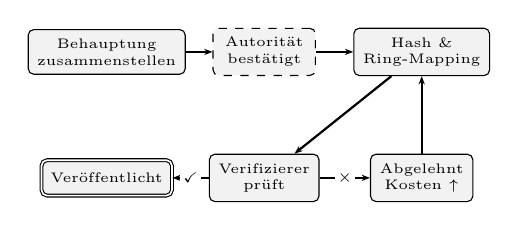
\begin{tikzpicture}[
    stp/.style={draw, rounded corners=2pt, minimum width=1.3cm, minimum height=0.45cm, align=center, font=\tiny, fill=black!5},
    arr/.style={-{Stealth[length=3pt]}, thick},
    lbl/.style={font=\tiny, fill=white, inner sep=1pt}
]
\node[stp] (comp) at (0,0) {Behauptung\\zusammenstellen};
\node[stp, dashed] (auth) at (2.0,0) {Autorität\\bestätigt};
\node[stp] (hash) at (4.0,0) {Hash \&\\Ring-Mapping};
\node[stp] (ver) at (2.0,-1.6) {Verifizierer\\prüft};
\node[stp, double] (pub) at (0,-1.6) {Veröffentlicht};
\node[stp] (rej) at (4.0,-1.6) {Abgelehnt\\Kosten $\uparrow$};

\draw[arr] (comp) -- (auth);
\draw[arr] (auth) -- (hash);
\draw[arr] (hash) -- (ver);
\draw[arr] (ver) -- node[lbl] {\checkmark} (pub);
\draw[arr] (ver) -- node[lbl] {$\times$} (rej);
\draw[arr] (rej) -- ++(0,0.8) -| (hash);
\end{tikzpicture}
\caption{Lebenszyklus einer Behauptung mit Iterationsschleife.}
\label{fig:lifecycle}
\end{figure}

\subsection{Verhältnis zu W3C DID Core}

Das Identitätsmodell des RSN ist eine echte Obermenge der W3C-DID-Core-Spezifikation~\cite{did2022}. Alle RSN-DIDs sind gültige W3C-DIDs. Die RSN-spezifischen Erweiterungen sind als DID-Dokumenteigenschaften kodiert, die in einer eigenen DID-Methodenspezifikation definiert sind und mit bestehender Infrastruktur wie ION~\cite{buchner2021} und Ceramic~\cite{ceramic2023} kompatibel sind.

% ============================================================
% 5. VERIFICATION AND PROPAGATION
% ============================================================
\section{Informationsverifizierung und -verbreitung}

\subsection{Kosten des Informationseintrags}

Das ökonomische Kernprinzip des RSN ist die Asymmetrie zwischen Lesen und Schreiben. Das Lesen von Reputationsdaten nähert sich für Teilnehmer, die Teil des DID-Netzwerks sind und über einen ihrer Reputation angemessenen Zugang verfügen, den marginalen Kosten von null---Neulinge müssen sich einen breiteren Zugang schrittweise verdienen (siehe Anti-Leeching). Schreiben---verstanden als die dauerhafte Materialisierung von Reputation in das Netzwerk, nicht als einmaliger technischer Akt---erfordert nachweisbare kumulative Investitionen über drei Dimensionen: \textbf{Zeit} (Lebensjahre, die auf konsistentes Verhalten, erfüllte Verpflichtungen und gepflegte Beziehungen verwendet werden), \textbf{Energie} (in ehrliches Handeln, die Pflege von Partnerschaften und langfristige Vertrauenswürdigkeit investierter Aufwand) und \textbf{Geld} (Investition in den eigenen Namen---berufliche Entwicklung, die Qualität der eigenen Arbeit, Wiedergutmachung für verursachte Schäden). Reputation kann nicht sofort erworben werden---sie ist das Ergebnis einer lebenslangen Akkumulation, die das System lediglich sichtbar und über Kontexte hinweg übertragbar macht. Die einmaligen technischen Kosten des Protokolls (kryptografische Signaturen, Verifiziergebühren) sind im Vergleich zu dieser zugrunde liegenden Investition vernachlässigbar.

\subsection{Sozialer Graph und Kontakttiefe}

Das RSN ist grundsätzlich ein soziales Netzwerk: Jede DID fügt Kontakte hinzu (andere DIDs), die die Verbindung zulassen. Diese Kontakte haben ihre eigenen Kontakte, und so weiter. Die algorithmische Verifiziersuche operiert innerhalb einer konfigurierbaren Tiefe $h$ verknüpfter Kontakte (z.\,B. $h=3$: die eigenen direkten Kontakte, deren Kontakte und die Kontakte der Kontakte). Diese Architektur erfordert keine einzige globale Blockchain---sie begünstigt naturgemäß die Entstehung von Gemeinschaften/Clustern mit Überschneidungen in andere Gemeinschaften. Jeder DID-Teilnehmer muss eine veröffentlichte \textbf{Richtlinie} haben---einen maschinenlesbaren Satz von Regeln, der bestimmt, wie eingehende Anfragen bewertet werden. Richtlinienverstöße werden im Netzwerk als negative Artefakte erfasst.

\subsection{Algorithmische Auswahl des Verifizierers}

Das Verifizierungsprotokoll verwendet konsistentes Hashing~\cite{karger1997} (Abb.~\ref{fig:verifier}). Verifizierung ist ein kostenpflichtiger Dienst: Verifizierer arbeiten gegen eine Gebühr und schaffen einen Markt, in dem der Wettbewerb Preisgestaltung, Geschwindigkeit und Zuverlässigkeit antreibt.

\textbf{Schritt 1.} Das Behauptungsdokument wird mit dem Hash-Ergebnis der vorherigen Iteration verkettet (oder $\varnothing$ bei der ersten Iteration) und gehasht:
\begin{equation}
\text{pos} = f_h(\text{claim} \| \text{prev\_hash})
\label{eq:hash}
\end{equation}

Der Algorithmus muss den \emph{vollständigen Pfad} aller vorherigen Anfragen und Antworten einbeziehen---nicht nur einen Hash der vorherigen Iteration. Die vollständige Antwort jedes Verifizierers (Annahme, Ablehnung, angebotener Preis, Begründung) wird an das wachsende Dokument angehängt und ist durch kryptografische Signaturen bei jedem Schritt verifizierbar.

\textbf{Schritt 2.} Der Hash wird auf $N$ Positionen auf dem konsistenten Hash-Ring abgebildet, gleichmäßig verteilt (z.\,B. für $N=4$: $+0^{\circ}, +90^{\circ}, +180^{\circ}, +270^{\circ}$). Von jeder Position aus wählt eine im Uhrzeigersinn verlaufende Suche die nächstgelegene DID als Verifizierer-Kandidat aus (Abb.~\ref{fig:multipoint}). $N$ ist ein variabler Parameter, der vom Prozentsatz der derzeit aktiven DIDs, der Tageszeit oder der historischen Netzwerk-Reaktionsfähigkeit abhängen kann.

\textbf{Schritt 3.} Der Verifizierer nimmt an (veröffentlicht, setzt Reputation ein) oder lehnt ab (Rückkehr zu Schritt~1 mit dem Ablehnungs-Hash). Wenn ein Knoten trotz deklariertem Online-Status nicht antwortet, muss die nächste Anfrage alle Antworten aller $N$ vorherigen Verifizierer-Kandidaten enthalten.

\textbf{Anti-Leeching.} Ziel-DIDs können Gebühren oder Zugangsbeschränkungen für Anfragen von neuen DIDs mit geringer Reputation festlegen. Dieser abgestufte Mechanismus (nicht binär) zwingt Neulinge dazu, durch echte Aktivität Reputation aufzubauen, bevor sie die Daten anderer frei konsumieren können.

\begin{figure}[ht]
\centering
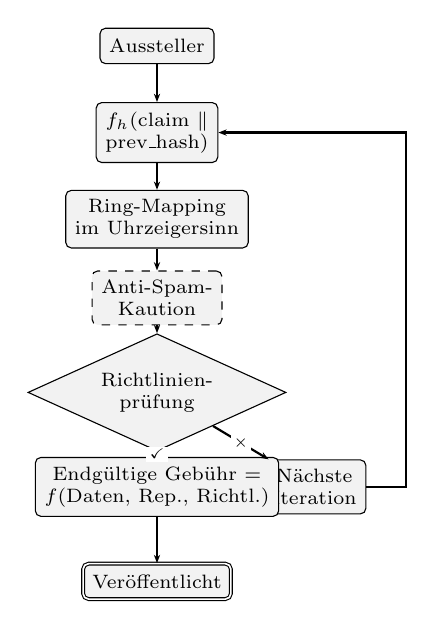
\begin{tikzpicture}[
    box/.style={draw, rounded corners=2pt, minimum width=1.3cm, minimum height=0.45cm, align=center, font=\scriptsize, fill=black!5},
    dec/.style={draw, diamond, aspect=2.2, minimum width=0.9cm, align=center, font=\scriptsize, fill=black!5},
    arr/.style={-{Stealth[length=3pt]}, thick},
    lbl/.style={font=\tiny, fill=white, inner sep=1pt}
]
\node[box] (iss) at (0,0) {Aussteller};
\node[box] (hash) at (0,-1.1) {$f_h$(claim $\|$\\prev\_hash)};
\node[box] (ring) at (0,-2.2) {Ring-Mapping\\im Uhrzeigersinn};
\node[box, dashed] (spam) at (0,-3.2) {Anti-Spam-\\Kaution};
\node[dec] (check) at (0,-4.4) {Richtlinien-\\prüfung};
\node[box] (rej) at (2,-5.6) {Nächste\\Iteration};
\node[box] (fee) at (0,-5.6) {Endgültige Gebühr =\\$f$(Daten, Rep., Richtl.)};
\node[box, double] (pub) at (0,-6.8) {Veröffentlicht};

\draw[arr] (iss) -- (hash);
\draw[arr] (hash) -- (ring);
\draw[arr] (ring) -- (spam);
\draw[arr] (spam) -- (check);
\draw[arr] (check) -- node[lbl] {$\times$} (rej);
\draw[arr] (check) -- node[lbl] {\checkmark} (fee);
\draw[arr] (fee) -- (pub);
\draw[arr] (rej.east) -- ++(0.5,0) |- (hash.east);
\end{tikzpicture}
\caption{Protokoll zur Auswahl des Verifizierers. Die Anti-Spam-Kaution ist optional und kann erstattungsfähig sein. Die endgültige Gebühr wird nur bei Annahme gezahlt.}
\label{fig:verifier}
\end{figure}

Jede Ablehnung hängt die vollständige Antwort des Verifizierers (einschließlich Gründe und Bedingungen) an das Behauptungsdokument an und erweitert dessen Inhalt. Aus dem erweiterten Dokument wird nichtdeterministisch ein neuer Hash berechnet, der auf eine andere Ringposition abgebildet wird und einen anderen Verifizierer auswählt. Die Dokumentation des vollständigen Pfades ist obligatorisch---der Aussteller kann den nächsten Verifizierer weder vorhersagen noch beeinflussen. Wenn ein Verifizierer eine Anfrage trotz kompatibler deklarierter Richtlinie ignoriert, halten Zeugen (sofern vorhanden) dies fest, und der Aussteller kann bei der endgültigen Veröffentlichung Zeugenbeweise beifügen.

\begin{figure}[ht]
\centering
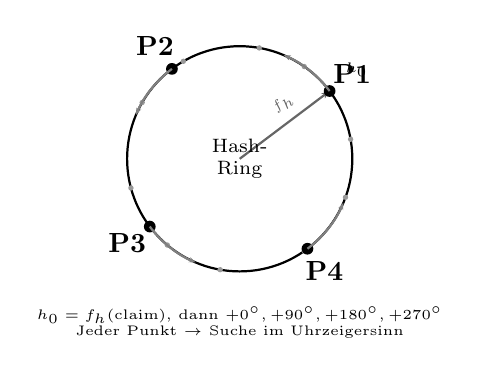
\begin{tikzpicture}[scale=0.65]
% Ring
\draw[thick] (0,0) circle (2.2cm);
% DID nodes on ring
\foreach \a in {10,55,80,120,150,195,230,260,305,340} {
  \fill[black!40] (\a:2.2) circle (1.5pt);
}
% Hash offset arrow pointing to initial position
\draw[-{Stealth[length=3pt]}, thick, black!60] (0,0) -- node[font=\tiny,above,sloped,pos=0.6] {$f_h$} (37:2.2);
\fill[black] (37:2.2) circle (2pt);
\node[font=\tiny,anchor=south west] at (37:2.35) {$h_0$};
% N=4 points offset from h0 by +0, +90, +180, +270
\foreach \offset/\l in {0/P1,90/P2,180/P3,270/P4} {
  \pgfmathsetmacro{\ang}{37+\offset}
  \node[fill=black, circle, inner sep=1.5pt] (p\offset) at (\ang:2.2) {};
  \node[font=\tiny,font=\bfseries] at (\ang:2.75) {\l};
  % clockwise search arc
  \draw[-{Stealth[length=2.5pt]}, thick, gray] (\ang:2.2) arc (\ang:\ang+30:2.2);
}
\node[font=\scriptsize, align=center] at (0,0) {Hash-\\Ring};
\node[font=\tiny, align=center] at (0,-3.2) {$h_0 = f_h(\text{claim})$, dann $+0^{\circ},+90^{\circ},+180^{\circ},+270^{\circ}$\\Jeder Punkt $\rightarrow$ Suche im Uhrzeigersinn};
\end{tikzpicture}
\caption{Mehrpunkt-Auswahl ($N{=}4$). Der Hash $h_0$ legt den Versatz fest; 4 Punkte gleichmäßig von $h_0$ verteilt.}
\label{fig:multipoint}
\end{figure}

\subsection{Zeugenprotokoll}

Die Rolle des \textbf{Zeugen} bietet über ein kryptografisches Challenge-Code-Protokoll inkognito Rechenschaftspflicht für die Ehrlichkeit des Verifizierers:

\textbf{Schritt W1.} Der Anfragende signiert die Verifizierungsanfrage und sendet sie an $N_w$ Zeugen---Kontakte aus dem sozialen Netzwerk des Anfragenden oder spezialisierte Zeugendienstanbieter, die gegen eine Gebühr arbeiten.

\textbf{Schritt W2.} Jeder Zeuge $w_i$ signiert die gesamte signierte Anfrage, behält die ursprüngliche Signatur $\sigma_i$ und berechnet einen Challenge-Code $c_i = h(\sigma_i)$. Der Challenge-Code wird an die Anfrage angehängt.

\textbf{Schritt W3.} Die Anfrage, die nun $N_w$ Challenge-Codes trägt, wird an den Verifizierer gesendet. Der Verifizierer beobachtet die Codes, kann aber \emph{nicht feststellen}, wer die Zeugen sind oder ob die Codes echten Signaturen entsprechen.

\textbf{Schritt W4 (ehrlicher Verifizierer).} Antwortet der Verifizierer gemäß seiner deklarierten Richtlinie, bleiben die Challenge-Codes undurchsichtig. Zeugen werden niemals offengelegt. Es werden keine zusätzlichen Daten veröffentlicht.

\textbf{Schritt W5 (Richtlinienverstoß).} Verstößt der Verifizierer gegen seine Richtlinie (ignoriert die Anfrage, antwortet inkonsistent), hält der Anfragende die ursprünglichen Signaturen $\sigma_i$ der Zeugen. Diese können als Begleitdaten veröffentlicht werden: Jeder kann $c_i = h(\sigma_i)$ verifizieren und damit beweisen, dass der Zeuge anwesend war. Der Anfragende kann unabhängig veröffentlichen---der Verifizierer hat die Challenge-Codes in seiner Antwort bereits signiert.

\textbf{Die Bluff-Eigenschaft.} Der Anfragende kann für einige oder alle Challenge-Codes zufällige Werte einsetzen. Der Verifizierer kann echte Codes (gedeckt durch Autoritäten mit hoher Reputation) nicht von Rauschen unterscheiden. Diese \emph{Ungewissheit} ist der Durchsetzungsmechanismus: Jede Anfrage birgt das Risiko, dass eine angesehene Autorität inkognito zusieht. Die Kosten, diesen Druck aufrechtzuerhalten, liegen nahe null (Erzeugung von Zufallszahlen), während die potenziellen Kosten der Unehrlichkeit für den Verifizierer katastrophal sind. Ehrliches Verhalten wird selbst in Abwesenheit tatsächlicher Zeugen begünstigt.

\textbf{Autorität als Zeuge.} Eine Autorität, die eine Behauptung bestätigt, kann Zeugendienste bündeln: „Ich bestätige Ihre Behauptung und diene während der Verifizierung als Inkognito-Zeuge.“ Dies ist ein natürliches Geschäftsmodell---die Autorität verfügt bereits über den Kontext. Die beiden Rollen sind jedoch logisch unabhängig.

\subsection{Prinzip des teuren Radikalismus}

Drei Kostenkanäle verstärken sich gleichzeitig (Abb.~\ref{fig:radicalism}):

\textbf{Kanal 1: Iterationskosten.} Jede Ablehnung erzwingt eine neue Iteration, die Zeit und Ressourcen verbraucht. Lineares Wachstum.

\textbf{Kanal 2: Dokumentenaufblähung.} Jede Iteration fügt die vollständige Verifiziererantwort zum Behauptungsdokument hinzu. Das Wachstum ist linear, jedoch mit einem Basisversatz: Die anfängliche Nutzlast (Behauptungsinhalt, Bestätigung durch die Autorität, kryptografische Signaturen) hat bereits eine nicht triviale Größe $B_0$. Gesamtgröße nach $k$ Iterationen: $S(k) = B_0 + k \cdot \Delta$, wobei $\Delta$ die durchschnittliche Antwortgröße ist.

\textbf{Kanal 3: Risikoaufschlag des Verifizierers.} Risiko ist subjektiv. Der Verifizierer beurteilt, ob die deklarierten Richtlinien der anfragenden DID mit den eigenen kommerziellen, sozialen oder politischen Interessen des Verifizierers in Konflikt stehen. Der Aufschlag kann exponentiell mit der wahrgenommenen Distanz vom „Ideal“ des Verifizierers eskalieren: $P(d) = \alpha \cdot e^{\beta d}$, wobei $d$ die subjektive Distanzmetrik des Verifizierers ist. Jenseits einer persönlichen No-Go-Grenze kann der Verifizierer vollständig ablehnen.

\begin{figure}[ht]
\centering
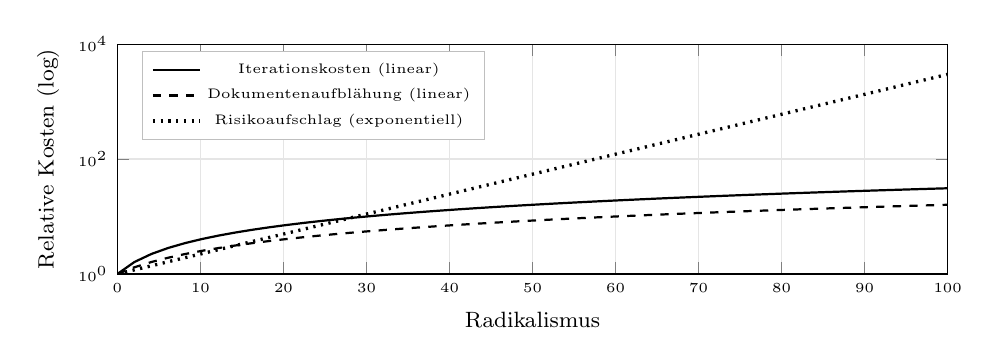
\begin{tikzpicture}
\begin{axis}[
    width=\columnwidth,
    height=4.5cm,
    xlabel={\footnotesize Radikalismus},
    ylabel={\footnotesize Relative Kosten (log)},
    ymode=log,
    xmin=0, xmax=100,
    ymin=1, ymax=10000,
    grid=major,
    grid style={gray!20},
    legend style={at={(0.03,0.97)},anchor=north west,font=\tiny,draw=gray!50},
    tick label style={font=\tiny},
    label style={font=\footnotesize},
]
\addplot[black, thick, domain=0:100, samples=50] {1 + 0.3*x};
\addlegendentry{Iterationskosten (linear)}
\addplot[black, thick, dashed, domain=0:100, samples=50] {1 + 0.15*x};
\addlegendentry{Dokumentenaufblähung (linear)}
\addplot[black, thick, dotted, line width=1.2pt, domain=0:100, samples=100] {exp(0.08*x)};
\addlegendentry{Risikoaufschlag (exponentiell)}
\end{axis}
\end{tikzpicture}
\caption{Kosteneskalation über drei Kanäle. Der Risikoaufschlag dominiert bei hohem Radikalismus.}
\label{fig:radicalism}
\end{figure}

Entscheidend ist: Dies ist keine Zensur. Keine Behauptung ist verboten. Das System bepreist das Risiko (Tabelle~\ref{tab:costs}).

\begin{table}[ht]
\centering
\caption{Kostenvergleich über verschiedene Behauptungstypen.}
\label{tab:costs}
\footnotesize
\begin{tabular}{@{}lcccc@{}}
\toprule
\textbf{Typ} & \textbf{Iter.} & \textbf{Dok.} & \textbf{Gebühr} & \textbf{Gesamt} \\
\midrule
Glaubwürdig & $k_{\min}$ & $B_0$ & $P_{\min}$ & Niedrig \\
Kontrovers & $k_{\text{med}}$ & $B_0{+}k\Delta$ & $\alpha e^{\beta d}$ & Mittel \\
Radikal & $k_{\max}$ & $\gg B_0$ & $\gg P_{\min}$ & Sehr hoch \\
Betrügerisch & $\to\infty$ & --- & --- & Unveröffentlichbar \\
\bottomrule
\end{tabular}
\end{table}

% ============================================================
% 6. REPUTATION AND RISK
% ============================================================
\section{Reputation und Risikobewertung}

\subsection{Modell der Reputationsakkumulation}

Reputation weist drei Eigenschaften auf: \textbf{langsame Akkumulation} (schrittweises Wachstum durch konsistentes Verhalten), \textbf{schnelle Zerstörung} (ein einziger Betrug kann den Score katastrophal senken) und \textbf{individuelle Bewertung} (jede konsumierende Partei kann ihre eigene Aggregationsfunktion anwenden).

\subsection{Reputable Autoritäten}

Eine reputable Autorität prüft Behauptungen und mitunterzeichnet sie, sofern sie überzeugt ist---und setzt dabei ihre eigene Reputation ein (Abb.~\ref{fig:authority}). Die Asymmetrie ist beabsichtigt: Reputation zu gewinnen ist langsam (schrittweise $+\delta$ pro ehrlicher Bestätigung), während ihr Verlust katastrophal ist ($-\Delta \gg \delta$ pro falscher Bestätigung; veranschaulichend etwa $+2\%$ gegenüber $-70\%$). Die optimale Strategie besteht immer darin, verdächtige Behauptungen abzulehnen. Die konkreten Werte von $\delta$ und $\Delta$ sind Systemparameter.

\begin{figure}[ht]
\centering
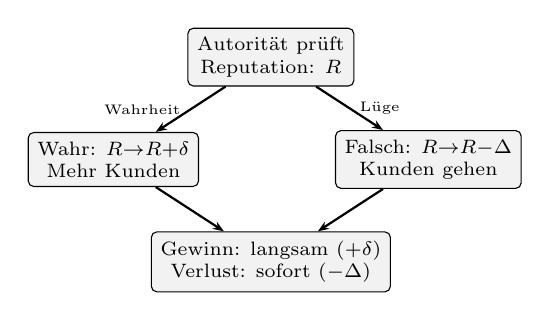
\begin{tikzpicture}[
    box/.style={draw, rounded corners=2pt, minimum width=2cm, minimum height=0.6cm, align=center, font=\scriptsize, fill=black!5},
    arr/.style={-{Stealth[length=4pt]}, thick}
]
\node[box] (exam) at (0,0) {Autorität prüft\\Reputation: $R$};
\node[box] (true) at (-2,-1.3) {Wahr: $R{\to}R{+}\delta$\\Mehr Kunden};
\node[box] (false) at (2,-1.3) {Falsch: $R{\to}R{-}\Delta$\\Kunden gehen};
\node[box] (insight) at (0,-2.6) {Gewinn: langsam ($+\delta$)\\Verlust: sofort ($-\Delta$)};

\draw[arr] (exam) -- node[left,font=\tiny] {Wahrheit} (true);
\draw[arr] (exam) -- node[right,font=\tiny] {Lüge} (false);
\draw[arr] (true) -- (insight);
\draw[arr] (false) -- (insight);
\end{tikzpicture}
\caption{Reputable Autorität---asymmetrische Anreize.}
\label{fig:authority}
\end{figure}

\subsection{Mehrdimensionale Reputation}

Reputation ist kein Skalar, sondern ein Vektor über mehrere Dimensionen: finanzielle Zuverlässigkeit, persönliche Integrität, fachliche Kompetenz, bürgerschaftliches Engagement und andere (Abb.~\ref{fig:reputation-radar}). Verschiedene Bewertungsanbieter projizieren diesen Vektor je nach Kontext unterschiedlich---ein Kreditgeber priorisiert die finanzielle Zuverlässigkeit, ein Arbeitgeber die fachliche Kompetenz, ein Nachbar das bürgerschaftliche Verhalten. Es gibt keinen einzigen „richtigen“ Reputationsscore; nur Perspektiven.

\begin{figure}[ht]
\centering
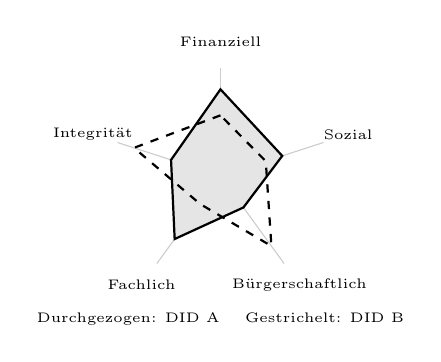
\begin{tikzpicture}[scale=0.55]
\foreach \a/\l in {90/Finanziell,162/Integrität,234/Fachlich,306/Bürgerschaftlich,18/Sozial} {
  \draw[gray!40] (0,0) -- (\a:2.5);
  \node[font=\tiny, align=center] at (\a:3.1) {\l};
  \foreach \r in {0.8,1.6,2.4} {
    \fill[black!15] (\a:\r) circle (0.5pt);
  }
}
\draw[thick, fill=black!10] (90:2.0) -- (162:1.2) -- (234:1.8) -- (306:0.9) -- (18:1.5) -- cycle;
\draw[thick, dashed] (90:1.4) -- (162:2.1) -- (234:0.8) -- (306:2.0) -- (18:1.1) -- cycle;
\node[font=\tiny] at (0,-3.3) {Durchgezogen: DID A \quad Gestrichelt: DID B};
\end{tikzpicture}
\caption{Mehrdimensionale Reputationsvektoren. Verschiedene DIDs weisen unterschiedliche Profile über die Dimensionen hinweg auf.}
\label{fig:reputation-radar}
\end{figure}

\subsection{Demokratisierte Risikobewertung}

Das RSN demokratisiert die systematische Risikobewertung---eine Fähigkeit, die derzeit bei Finanzinstituten konzentriert ist, aber weit über das Bankwesen hinaus anwendbar ist. Industriekonglomerate, die die Zuverlässigkeit von Lieferanten bewerten, Versicherungsunternehmen, die Verhaltensrisiken bepreisen, Due Diligence bei Fusionen und Übernahmen, Schätzung der Lebensdauer von Anlagen in der Fertigung---überall dort, wo das Risiko der Gegenpartei bewertet werden muss, bietet das RSN eine dezentrale, marktgetriebene Alternative. Ein Markt für Interpretationsdienste übersetzt rohe mehrdimensionale Reputationsdaten in handlungsleitende Zusammenfassungen und macht die Bewertung der Gegenpartei für jeden Teilnehmer zu marginalen Kosten zugänglich.

% ============================================================
% 7. CONSENSUS AND DISPUTE RESOLUTION
% ============================================================
\section{Konsens und Streitbeilegung}

\subsection{Modell dezentraler Gerechtigkeit}

Das RSN formuliert Gerechtigkeit als bilaterales Verhandlungsproblem neu. Die Drohung eines dauerhaften, verifizierbaren Reputationsschadens ist ein wirksameres Abschreckungsmittel als Gerichtsverfahren, die sich die geschädigte Partei nicht leisten kann.

\subsection{Emergenter Konsens}

Jeder Teilnehmer unterhält eine persönliche Zufriedenheitsschwelle. Der aggregierte Konsens des Netzwerks entsteht als statistischer Durchschnitt tausender bilateraler Verhandlungen (Abb.~\ref{fig:consensus}). Eine Reaktion weit oberhalb des Konsenses (barbarisch) ist teuer zu veröffentlichen. Eine Reaktion nahe dem Konsens (verhältnismäßig) ist günstig. Der Konsens ist keine Regel---er ist ein Preissignal.

\begin{figure}[ht]
\centering
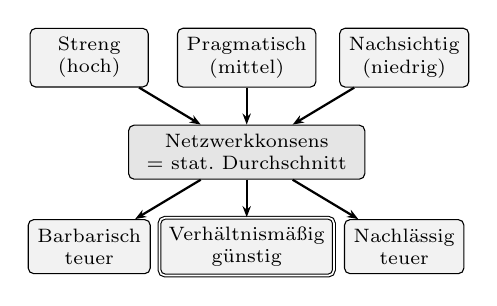
\begin{tikzpicture}[
    person/.style={draw, rounded corners=2pt, minimum width=1.5cm, minimum height=0.5cm, align=center, font=\scriptsize, fill=black!5},
    arr/.style={-{Stealth[length=4pt]}, thick}
]
\node[person] (a) at (-2,0) {Streng\\(hoch)};
\node[person] (b) at (0,0) {Pragmatisch\\(mittel)};
\node[person] (c) at (2,0) {Nachsichtig\\(niedrig)};
\node[person, fill=black!10, minimum width=3cm] (cons) at (0,-1.2) {Netzwerkkonsens\\= stat.\ Durchschnitt};
\node[person] (exp) at (-2,-2.4) {Barbarisch\\teuer};
\node[person, double] (prop) at (0,-2.4) {Verhältnismäßig\\günstig};
\node[person] (neg) at (2,-2.4) {Nachlässig\\teuer};

\draw[arr] (a) -- (cons);
\draw[arr] (b) -- (cons);
\draw[arr] (c) -- (cons);
\draw[arr] (cons) -- (exp);
\draw[arr] (cons) -- (prop);
\draw[arr] (cons) -- (neg);
\end{tikzpicture}
\caption{Emergenter Konsens aus individuellen Zufriedenheitsschwellen.}
\label{fig:consensus}
\end{figure}

\subsection{Kalibrierung der Bestrafung}

Jeder DID-Inhaber deklariert öffentlich Reaktionen auf bestimmte Kategorien von Fehlverhalten. Unverhältnismäßig harte oder milde Deklarationen ziehen negative Reputationssignale nach sich. Verhältnismäßige Deklarationen werden reibungslos akzeptiert---ein sich selbst kalibrierendes Bestrafungssystem.

Konsensdeklarationen unterliegen selbst der Heuchelei-Erkennung: sich deklarativ zu einer Konsensposition zu verpflichten und dabei inkonsistent zu handeln, stellt ein Reputationsvergehen dar, das schwerer wiegt als die zugrunde liegende Abweichung, da es eine absichtliche Täuschung belegt.

\subsection{Delegation}

Alle Aktivitäten innerhalb einer DID können---mit einer Ausnahme---an eine andere DID delegiert werden. \textbf{Die Subjekt-Rolle---die DID, um deren Verhalten es in der Behauptung geht---kann nicht delegiert werden; sie ist nicht übertragbar an den Identitätsinhaber gebunden, auf den sich die Behauptung bezieht.} Die anderen aktiven Rollen---Aussteller, Autorität, Zeuge, Verifizierer---können an eine benannte Delegat-DID übertragen werden, sei es zur Verifizierung, zur Übermittlung von Behauptungen, zur Konsensbeteiligung oder zur Streitbeilegung. Die Delegation ist jederzeit widerrufbar. Dies ermöglicht Spezialisierung (z.\,B. professionelle Verifizierungsdienste), während der Inhaber die letztliche Kontrolle und Verantwortung behält. Delegation gilt im gesamten System und ist für die Skalierbarkeit unerlässlich.

\subsection{Von individueller Moral zum emergenten Gesellschaftsvertrag}

Die deklarierte Richtlinie jeder DID stellt eine Formalisierung der individuellen Moral dar: was der Inhaber für akzeptabel hält, wie er auf bestimmte Verhaltensweisen reagiert, was er von Gegenparteien verlangt. Diese Richtlinien werden nicht von einem Systemgestalter auferlegt---sie werden von jedem Teilnehmer gewählt und in maschinenlesbarer Form ausgedrückt.

Diese Formalisierung ermöglicht eine dreistufige Emergenz. Erstens wird individuelle Moral als \textbf{Richtlinie} kodiert---ein Satz deklarierter Regeln, Schwellenwerte und Reaktionsfunktionen, deren Einhaltung sich die DID verpflichtet. Zweitens erzeugt die Gesamtheit aller Richtlinien über das Netzwerk hinweg eine \textbf{emergente Ethik}---statistisch beobachtbare Normen, die kein einzelner Teilnehmer entworfen hat, die aber aus der Interaktion tausender individueller moralischer Positionen entstehen~\cite{durkheim1893}. Drittens bilden diese emergenten Ethiken, ausgedrückt als geteilte Verhaltensnormen, die durch bilaterale Preissignale durchgesetzt werden, einen \textbf{messbaren Gesellschaftsvertrag}---kein theoretisches Konstrukt, das niemand unterzeichnet hat~\cite{rawls1971}, sondern ein empirisch beobachtbarer Satz von Regeln, der durch tatsächliches Verhalten gedeckt ist.

Dieser Prozess spiegelt Erkenntnisse der Theorie der moralischen Grundlagen wider~\cite{haidt2012}: Die menschliche Moral ist intuitiv, pluralistisch und kulturell variabel. Das RSN erfordert keinen moralischen Konsens als Eingabe; es erzeugt einen Verhaltenskonsens als Ausgabe. Der resultierende Gesellschaftsvertrag ist nicht statisch---er entwickelt sich weiter, während Teilnehmer beitreten, ausscheiden und ihre Richtlinien als Reaktion auf Netzwerk-Feedback anpassen. Anders als bei der klassischen Gesellschaftsvertragstheorie ist dieser Vertrag widerrufbar, beobachtbar und ohne einen Souverän durchsetzbar.

% ============================================================
% 8. ECONOMIC MODEL
% ============================================================
\section{Ökonomisches Modell}

Die vorangegangenen Abschnitte beschrieben ein Werkzeug---die Verifizierungsmechanismen, die Kostenstruktur und den emergenten Konsens des RSN. Dieser Abschnitt beschreibt eine Methodik zur Anwendung dieses Werkzeugs auf den fiskalischen und Governance-Übergang. Das Werkzeug ist von allgemeinem Zweck; die nachfolgende Methodik ist eine mögliche Anwendung.

\subsection{Anreizstruktur}

Reputation als Kapital schafft direkte Anreize für ehrliches Verhalten. Im Normalbetrieb bauen Teilnehmer auf natürliche Weise Reputation durch alltägliche Transaktionen und erfüllte Verpflichtungen auf. Die primäre Ausgabe entfällt auf \emph{negative} Behauptungen---die Erfassung von Schaden, der von anderen verursacht wurde. Diese Asymmetrie fördert nützliches, zuverlässiges Verhalten: Ehrlich zu sein kostet nichts zusätzlich, während schädliches Verhalten eine dokumentierte Spur schafft, deren Erhaltung andere sich etwas kosten lassen. Heuchelei---Regeln zu deklarieren, ohne sie zu befolgen---ist der teuerste Fehlermodus, da sie eine absichtliche Täuschung belegt.

\subsection{Paralleles Fiskalsystem}

Drei Komponenten ermöglichen Wettbewerbsdruck: (1)~\textbf{Einfache Steuer}---ein einziger proportionaler Satz ohne Ausnahmen, anfänglich marginal unter dem bestehenden effektiven Satz; (2)~\textbf{Elektronische Ausgabenregistrierung (ESR)}---eine Umkehrung des tschechischen EET-Modells, sodass Bürger die staatlichen Ausgaben überwachen; (3)~\textbf{Bürgergesteuerte Steuerzuweisung}---beginnend bei einigen Prozent im ersten Jahr und nach einem Jahrzehnt irgendwo zwischen einem niedrigen zweistelligen Bereich und einer vollständigen Migration zu einem bürgergesteuerten System erreichend, je nach Adoptionsrate. Das tatsächliche Tempo hängt von der Geschwindigkeit ab, mit der freimarktwirtschaftliche Alternativen zu staatlichen Diensten entstehen, sowie von der Bereitschaft des Staates, mit dem Übergang zu kooperieren; die Funktion der Zeit muss nicht linear sein, und es gibt keinen Grund, eine Obergrenze dafür festzulegen, wo die Adoption letztlich ankommen kann.

% ============================================================
% 9. MIGRATION PATH
% ============================================================
\section{Migrationspfad}

Die Migration verläuft über drei Phasen (Abb.~\ref{fig:migration}): \textbf{Phase~1: Overlay} (RSN als informationelle Schicht, Staat ist alleiniger Anbieter), \textbf{Phase~2: Wettbewerb} (RSN bietet funktionale Alternativen, Nutzung eines Doppelsystems) und \textbf{Phase~3: Übergang} (RSN übertrifft staatliche Entsprechungen, freiwillige Migration). Der Übergang ist in jeder Phase umkehrbar.

\begin{figure}[ht]
\centering
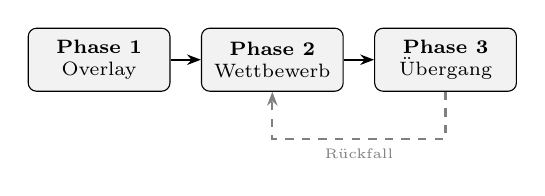
\begin{tikzpicture}[
    phase/.style={draw, rounded corners=3pt, minimum width=1.8cm, minimum height=0.8cm, align=center, font=\scriptsize, fill=black!5},
    arr/.style={-{Stealth[length=5pt]}, thick}
]
\node[phase] (p1) at (0,0) {\textbf{Phase 1}\\Overlay};
\node[phase] (p2) at (2.2,0) {\textbf{Phase 2}\\Wettbewerb};
\node[phase] (p3) at (4.4,0) {\textbf{Phase 3}\\Übergang};

\draw[arr] (p1) -- (p2);
\draw[arr] (p2) -- (p3);
\draw[arr, dashed, gray] (p3.south) -- ++(0,-0.6) -| node[below,font=\tiny,pos=0.25] {Rückfall} (p2.south);
\end{tikzpicture}
\caption{Dreiphasige Migration---in jeder Phase umkehrbar.}
\label{fig:migration}
\end{figure}

Der primäre Druckmechanismus ist fiskalisch: Wenn bedingte Steuerzahler eine „wirtschaftlich bedeutsame Minderheit $X$“ erreichen---eine Gruppe, die groß genug ist, dass Repression gegen sie nicht triviale wirtschaftliche Schäden verursacht und ziviler Ungehorsam zu einer glaubwürdigen Bedrohung wird---tritt der Staat in Verhandlungen ein. Zur Veranschaulichung verwenden wir $X \approx 15\%$ des BIP, aber die tatsächliche Schwelle hängt von der jeweiligen Volkswirtschaft ab.

% ============================================================
% 10. SECURITY ANALYSIS
% ============================================================
\section{Sicherheitsanalyse}

Wir betrachten fünf Kategorien von Angreifern: einzelne schlechte Akteure, organisierte Gruppen, unternehmerische Angreifer, staatliche Angreifer und Angreifer auf Protokollebene.

\textbf{Sybil-Resistenz}~\cite{douceur2002}. Der Aufbau von Reputation erfordert anhaltende, verifizierbare Interaktion. Die Kosten eines erfolgreichen Sybil-Angriffs skalieren linear mit der Anzahl gefälschter Identitäten und quadratisch mit dem angestrebten Reputationsniveau. Der parallele Betrieb mehrerer DIDs ist möglich, aber konstruktionsbedingt teuer---jede Identität muss unabhängig Reputation durch echte Aktivität akkumulieren. In freien Gesellschaften schreckt diese Kosten von beiläufigem Missbrauch ab; in Diktaturen werden parallele DIDs zu einem Überlebenswerkzeug, das kompartimentierten Widerstand, konspirative Koordination und eine sicherere Navigation auf dem Schwarzmarkt ermöglicht.

\textbf{Kollusionsabwehr.} Muster gegenseitiger Bestätigung innerhalb geschlossener Gruppen sind durch Analyse des sozialen Graphen erkennbar. Reputationsaggregationsfunktionen gewichten Behauptungen aus eng geclusterten Quellen ab.

\textbf{Staatlicher Angreifer.} Onion-Routing, das Fehlen zentralisierter Infrastruktur und die Verteilung der Verifizierer-Rolle über die Teilnehmerbasis stellen sicher, dass eine Unterdrückung Maßnahmen erfordert, die in keinem Verhältnis zu irgendeinem Nutzen stehen.

\textbf{Datenschutz vs.\ Rechenschaftspflicht.} Pseudonymität---ein Mittelweg zwischen Anonymität und Identitätsoffenlegung---erlaubt DIDs, bedeutsame Reputation zu akkumulieren, ohne die reale Identität des Inhabers preiszugeben.

% ============================================================
% 11. PRIVACY
% ============================================================
\section{Datenschutzüberlegungen}

Das Datenschutzmodell des RSN beruht auf Pseudonymität. Der Inhaber kontrolliert die Identitätsoffenlegung: minimal (reines Pseudonym), selektiv (bestimmte Berechtigungsnachweise verknüpft) oder vollständig (rechtliche Identität zugeordnet). Veröffentlichte Behauptungen sind dauerhaft---das System unterstützt kontextuelle Korrektur, aber keine Löschung. Ein Inhaber kann eine kompromittierte DID aufgeben und neu beginnen, wobei er die angesammelte Reputation verwirkt.

% ============================================================
% 12. RELATED WORK
% ============================================================
\section{Verwandte Arbeiten}

Die W3C-DID-Core-Spezifikation~\cite{did2022} und das Ceramic Network~\cite{ceramic2023} bilden die Identitätsgrundlage. EigenTrust~\cite{kamvar2003} demonstrierte eine verteilte Reputationsaggregation ohne zentrale Autorität. SBTs~\cite{weyl2022} führten nicht übertragbare soziale Token ein. Das RSN unterscheidet sich in seiner Betonung ökonomischer Kosten als Qualitätsfilter und in seinem Mechanismus zur Bepreisung von Radikalismus.

DAOs~\cite{buterin2014} und quadratisches Abstimmen~\cite{buterin2019} demonstrierten die Machbarkeit dezentraler Governance. Das RSN leitet Konsens aus bilateralen Preisverhandlungen statt aus Abstimmungen ab.

Der Vorschlag stützt sich auf die anarcho-kapitalistische Theorie~\cite{rothbard1973,hoppe2001} für die private Diensterbringung, weicht jedoch in zwei entscheidenden Punkten ab: Er ist auf Boshaftigkeit und Vergeltungsimpulse ausgelegt, statt Rationalität anzunehmen, und schlägt einen schrittweisen Übergang statt einer Revolution vor. Das Konzept emergenter Gesellschaftsverträge hat Vorläufer in Hayeks Theorie der spontanen Ordnung~\cite{hayek1973}.

\textbf{Anarcho-Agorismus.} Das RSN teilt bedeutende Gemeinsamkeiten mit der agoristischen Gegenökonomie~\cite{konkin2006}---insbesondere die Betonung des Aufbaus paralleler Institutionen und des freiwilligen Austauschs. Der Agorismus neigt jedoch dazu, rationales Eigeninteresse als hinreichenden Koordinationsmechanismus anzunehmen, und es fehlt ihm oft ein konkreter Migrationspfad von bestehenden Staatsstrukturen. Das RSN integriert ausdrücklich nicht-rationale Verhaltensneigungen und stellt einen fiskalischen Druckmechanismus für einen schrittweisen Übergang bereit.

\textbf{Meritokratie.} Das RSN könnte eine erste funktionale Beschreibung dessen darstellen, wie Meritokratie~\cite{young1958} als systemische Eigenschaft statt als Schlagwort entstehen kann. Traditionelle meritokratische Systeme scheitern, weil sie eine zentrale Autorität erfordern, um „Verdienst“ zu definieren und durchzusetzen. Im RSN entsteht Verdienst aus bilateralen Bewertungen: Wer Wert liefert, akkumuliert Reputation; kein Komitee entscheidet, wer Verdienst hat.

\textbf{Eigentum als Privileg.} Das RSN weicht grundlegend von anarcho-kapitalistischen und österreichisch-schulischen Behandlungen von Eigentumsrechten als natürlich und absolut ab. Im RSN-Rahmenwerk ist Eigentum ein \emph{Privileg}---eine gesellschaftliche Anerkennung, die in extremen Fällen von der Gemeinschaft zurückgezogen werden kann, wenn ein Teilnehmer geteilte Normen grundlegend verletzt (Verrat, Weigerung, die Gemeinschaft in einer existenziellen Krise zu verteidigen, systematische Ausbeutung). Dies ist keine staatliche Enteignung, sondern ein Entzug gesellschaftlicher Anerkennung durch das Netzwerk bilateraler Beziehungen.

% ============================================================
% 13. LIMITATIONS
% ============================================================
\section{Diskussion und Grenzen}

\textbf{Kaltstart.} Der Wert des RSN hängt von Netzwerkeffekten ab; frühe Anwender sehen sich mit begrenztem Nutzen konfrontiert, bis die Teilnahme eine Schwelle erreicht. Doch selbst in frühen Stadien dient das DID-Netzwerk als nützliche ergänzende Informationsquelle. Es ist zu erwarten, dass sich die frühe Reputationsbewertung und Autoritätseinschätzung mit zunehmender Ausgereiftheit schrittweise entwickeln.

\textbf{Anti-Leeching und Zugangskontrolle.} Ziel-DIDs können abgestufte Gebühren und Zugangsbeschränkungen für Anfragen von DIDs mit niedriger Reputation verhängen. Dies ist nicht binär, sondern eine kontinuierliche Skala: Je weniger Reputation eine anfragende DID hat, desto weniger Informationen erhält sie, desto länger wartet sie und desto mehr zahlt sie. Dieser Mechanismus fördert echte Teilnahme gegenüber passivem Konsum.

\textbf{Ungleichheit des Zugangs.} Die Kosten der Veröffentlichung von Behauptungen können legitime Beschwerden wirtschaftlich benachteiligter Teilnehmer herausfiltern. Abhilfe: Jeder Teilnehmer dient gleichzeitig als potenzieller Verifizierer (oder delegiert diese Rolle) und verdient Verifiziergebühren. Über einen ausreichenden Zeithorizont sollte sich ein nicht-radikaler Teilnehmer der finanziellen Neutralität annähern---die Verifiziereinnahmen gleichen die Veröffentlichungskosten näherungsweise aus. Dies ist eine statistische Erwartung, keine Garantie.

\textbf{Reputationsungleichheit.} Frühe Anwender akkumulieren Vorteile, die Barrieren für Nachzügler schaffen können. Die Reputationsbewertung wird jedoch von Drittanbietern durchgeführt, die sich dafür entscheiden können, den Vorteil des Erstanwenders durch ihre Aggregationsalgorithmen abzumildern. Als Erster über eine gute Reputation zu verfügen, ist ein legitimer komparativer wirtschaftlicher Vorteil---und das ist beabsichtigt.

\textbf{Offene Fragen.} Optimale Kostenfunktionen, Aggregationsstandards, Protokoll-Governance und die Interaktion mit KI-generierten synthetischen Reputationsdaten bleiben Bereiche für künftige Arbeiten.

Diese Arbeit erhebt nicht den Anspruch, dass das RSN unter allen Umständen optimale Ergebnisse liefern wird. Sie beansprucht, dass das RSN eine \emph{machbare} Alternative darstellt---technisch umsetzbar, wirtschaftlich selbsttragend und sozial kompatibel mit menschlichen Verhaltensneigungen, wie sie tatsächlich sind.

% ============================================================
% 14. CONCLUSION
% ============================================================
\section{Schlussfolgerung}

Diese Arbeit hat das Reputationsnetzwerk vorgestellt, ein dezentrales Protokoll, das einen pseudonymen, verifizierbaren Reputationsaustausch ermöglicht. Das Prinzip des teuren Radikalismus stellt sicher, dass betrügerische Behauptungen ohne Zensur aus dem Markt gepreist werden. Der vorgeschlagene Migrationspfad ermöglicht einen schrittweisen, umkehrbaren Übergang von bestehenden Institutionen. Der Entwurf integriert die menschliche Natur, wie sie ist---einschließlich Kleinlichkeit, Boshaftigkeit und dem Verlangen nach vergeltender Genugtuung---, statt eine ideologische Transformation zu verlangen. Das Ergebnis ist keine Utopie, sondern ein System, in dem Gerechtigkeit zugänglich ist, Reputation verdient wird und die Kosten des Fehlverhaltens von derjenigen Partei getragen werden, die es verursacht hat.

% ============================================================
% REFERENCES
% ============================================================
\bibliography{references}

\end{document}
